%Name: Template of COMP9020 Assignments
%Author:Jack
%Date: 14/08/2017
%Acknowledgement: This template is based on work of Brendan Trinh of UNSW MathSoc 2015
\documentclass[11pt, a4paper]{article}

\usepackage{amsmath} % Improves structure of typed out maths
\usepackage{mathtools} % Improves upon deficiencies of amsmath package
\usepackage{amssymb} % Adds some handy symbols to use.
\usepackage{amsthm} % Adds some neat formulas to use, e.g. \begin{proof} etc.

\usepackage[a4paper]{geometry} % Default page margins can be altered.
\usepackage{microtype} % Improves spacing between letters.
\usepackage{booktabs} % Improves tables. Can now create without vertical separators.
\usepackage{array} % Includes more options for arrays
\usepackage{paralist} % More flexible use of itemize, enumerate, etc.
\usepackage{graphicx} % Add images to your document
\usepackage{color} % Allows for the use of colours!
\usepackage{cleveref} % Better cross-referencing
\usepackage{hyperref} % For adding hyperlinks
\usepackage{fancyhdr} % Customise headers & footers in document
\usepackage{paralist}

\usepackage{url} % For adding url

\begin{document}
	\title{COMP9020 - Assignment 1}
	\author{Jack(z5129432)}
	\date{ 14ed August 2017 }
	\maketitle
	\graphicspath{{/}}

	\section*{Question 1}
	\begin{enumerate}[(a)]
		\item Show that: $\sum_{i=1}^{n}{i^2}=O(n^3)$\
		
		correct. $\sum_{i=1}^{n}{i^2} = \frac{n(n+1)(2n+1)}{6}$, which is $O(n^3)$\
		
		Related Nodes:\
		\begin{itemize}
			\item Arithmetic progression: SUM = $n\frac{(a_1 + a_n)}{2}$
			\item Geometric progression: SUM = $a_1\frac{1-r^n}{1-r}$
			\item Square number: SUM = $\frac{n(n+1)(2n+1)}{6}$
			\item Cubic number: SUM = $(\frac{n(n+1)}{2})^2$
		\end{itemize}
				
		\item\
		
		let $p(n) = n^c$, then $\log{p(n)} = \log{n^c} = c\log{n}$

		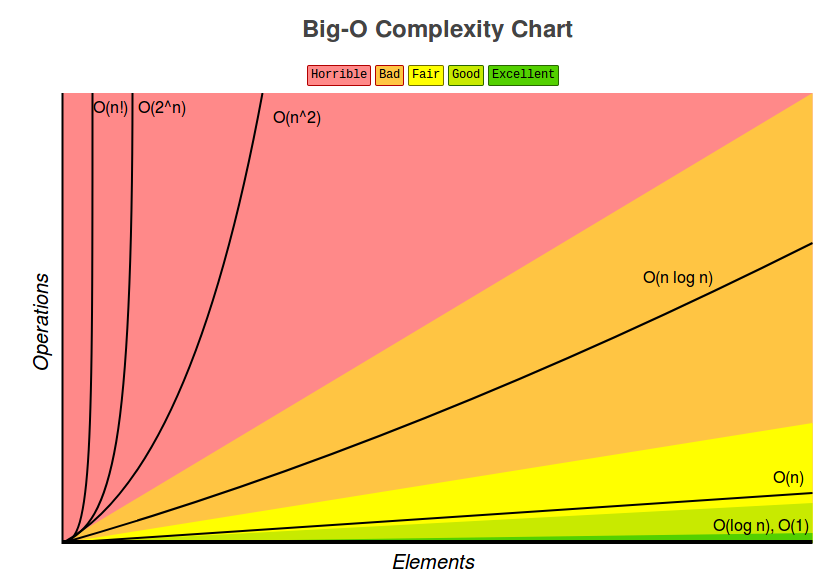
\includegraphics[scale=0.5]{bigo.png}
		\begin{itemize}
			\item O(1): constant
			\item O(logn): logarithmic
			\item O(n): linear
			\item O(nlogn): loglinear
			\item $O(n^c): polynomial$
			\item $O(c^n): exponential$
		\end{itemize}

		\item Show that $\sum_{i=1}^{n}{\log{i}} = O(n\log{n})$\
		
		$\sum_{i=1}^{n}{\log{i}} \leq \sum_{i=1}^{n}{\log{n}} = O(n\log{n})$

		\item Show that $\sum_{i=1}^{n}{\frac{i}{2^i}} = O(1)$\
		

	\end{enumerate}

\end{document}